\begin{figure}
\begin{tabular}{cc}
\begin{minipage}[t]{1in}
\begin{tabular}{l}
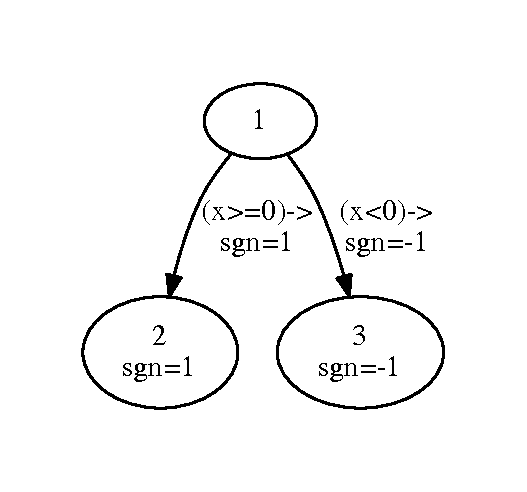
\includegraphics[width=1in,clip=true,trim = 20pt 20pt 30pt 20pt]{figures/sign} \\
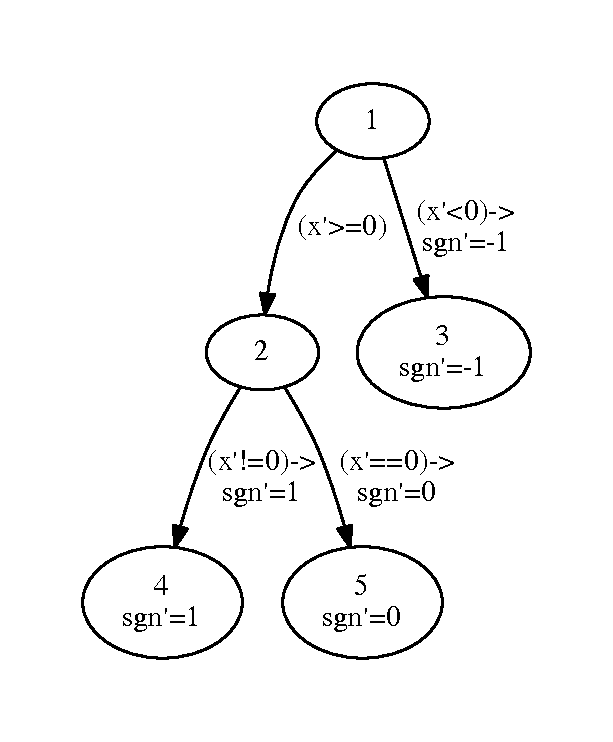
\includegraphics[width=1in,clip=true,trim = 20pt 20pt 30pt 20pt]{figures/sign-tag}
\end{tabular}
\end{minipage}
&
\begin{minipage}[t]{1in}
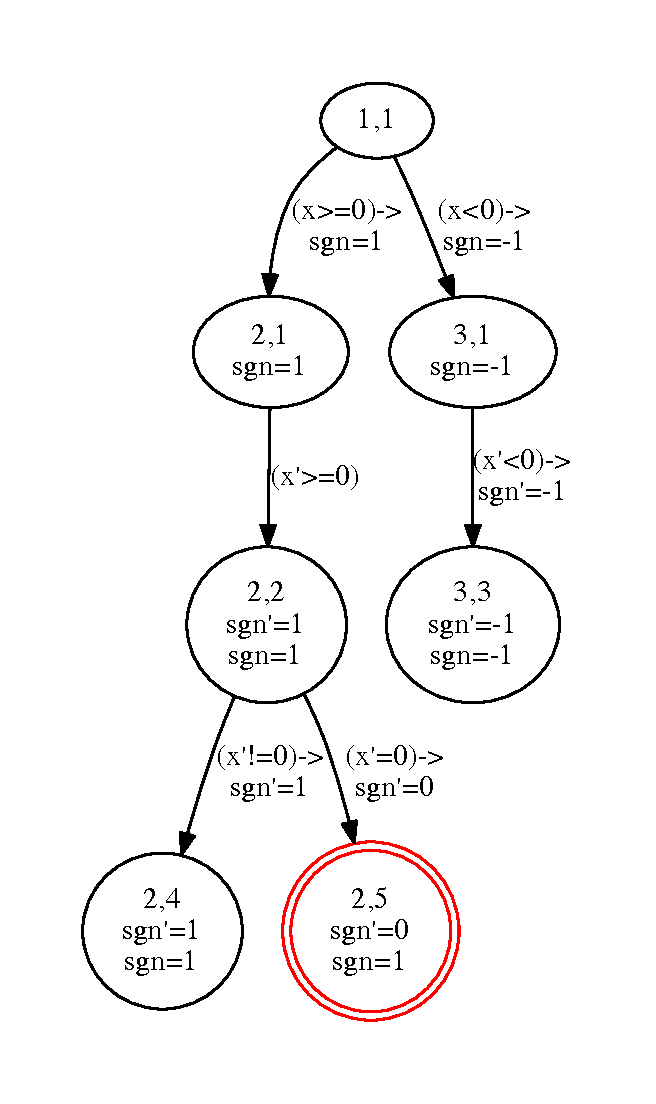
\includegraphics[width=1in,clip=true,trim = 20pt 20pt 30pt 20pt]{figures/sign-correlated}
\end{minipage}
\end{tabular}
\end{figure}


\begin{itemize}
\item $\asemp{v:=e} = l_{\times} \mapsto \{\langle ctx,\asemp{v:=e}_{\A{D}}(data) \rangle | (ctx,data) \in S \}$
\item $\asemp{g:=e} = l_{\times} \mapsto \{\langle \asemp{g:=true}_{\A{D}}(ctx),\asemp{e}_{\A{D}}(data) \rangle  | (ctx,data) \in S \} \cup \{ <\asemp{g:=false}_{\A{D}}(ctx),\asemp{\neg e}_{\A{D}}(data)> | (ctx,data) \in S \}$
\item $\asemp{\textbf{if} (g) \{s_{0}\} \textbf{else} \{s_{1}\}} = l_{\times} \mapsto \{\langle\asemp{g=true}_{\A{D}}(ctx),  \asemp{s_0}_{\A{D}}(data) \rangle | (ctx,data) \in S \} \cup
                                                                                      \{\langle \asemp{g=false}_{\A{D}}(ctx), \asemp{s_1}_{\A{D}}(data) \rangle | (ctx,data) \in S \}$
\item $\asemp{\textbf{goto} lab} = \A{\sigma}$
\end{itemize}


In this setting, as we advance through the analysis of $P$, we will accumulate the disjunction of all possible path constraints in its final state (this is similar to trace partitioning~\cite{MauborgneRival07}). At this point, as we continue to analyze $P'$, each disjunct representing a path in $P$ will be further conjuncted with all of $P'$ paths. This will produce a precise disjunction for differencing as each path in $P$ will be split and conjuncted with all of $P'$ paths, while avoiding considering conjunctions that disagree on input due to our input equivalence assumption.


A correlating abstraction is well suited for proving equivalence as it allows focusing on relationships between versions of variables while abstracting away other (numerical) information allowing us to scale better. Most importantly, such an abstraction guarantees that equivalence will be reported soundly: as in a separate analysis we abstracted $\langle sgn \mapsto -1 \rangle$ and $\langle sgn \mapsto 1 \rangle$ towards an interval $\langle sgn \mapsto [-1,1] \rangle$, and again for $sgn'$ values, separately, which cannot assure equivalence (and in fact shouldn't). We instead use correlating states: $s_1 = \langle sgn = sgn' \mapsto -1 \rangle$ and $s_2 = \langle sgn = sgn' \mapsto 1 \rangle$, which allow us to abstract as such $s_1 \sqcup s_2 = \langle sgn = sgn', sgn \mapsto [-1,1] \rangle$ so equivalence can be soundly assured.

%If we instead use disjunctive completion powerset domain~\cite{TODO} where the abstract state is a set of convex sub-states, and no merge is ever performed, this would yield a precise result that may be used for equivalence checking and differencing.  For instance, using such domain for $sign$ would yield: $\langle x < 0, sgn = -1 \rangle \vee \langle x \geq 0, sgn = 1 \rangle$ and for $sign'$: $\langle x < 0, sgn = -1 \rangle \vee \langle x > 0, sgn = 1 \rangle \vee \langle x = 0, sgn = 0 \rangle$. Further refining $sign$'s abstraction and splitting the $\langle x \geq 0, sgn = 1 \rangle$ constraint to $\langle x > 0, sgn = 1 \rangle \vee \langle x = 0, sgn = 0 \rangle$ would allow perfectly aligning the input constraints to produce the difference of $x=0,sgn=1,sgn'=0$ as depicted in \figref{SignComplete}.
%\begin{wrapfigure}{r}{0cm}
%\imagetop{
%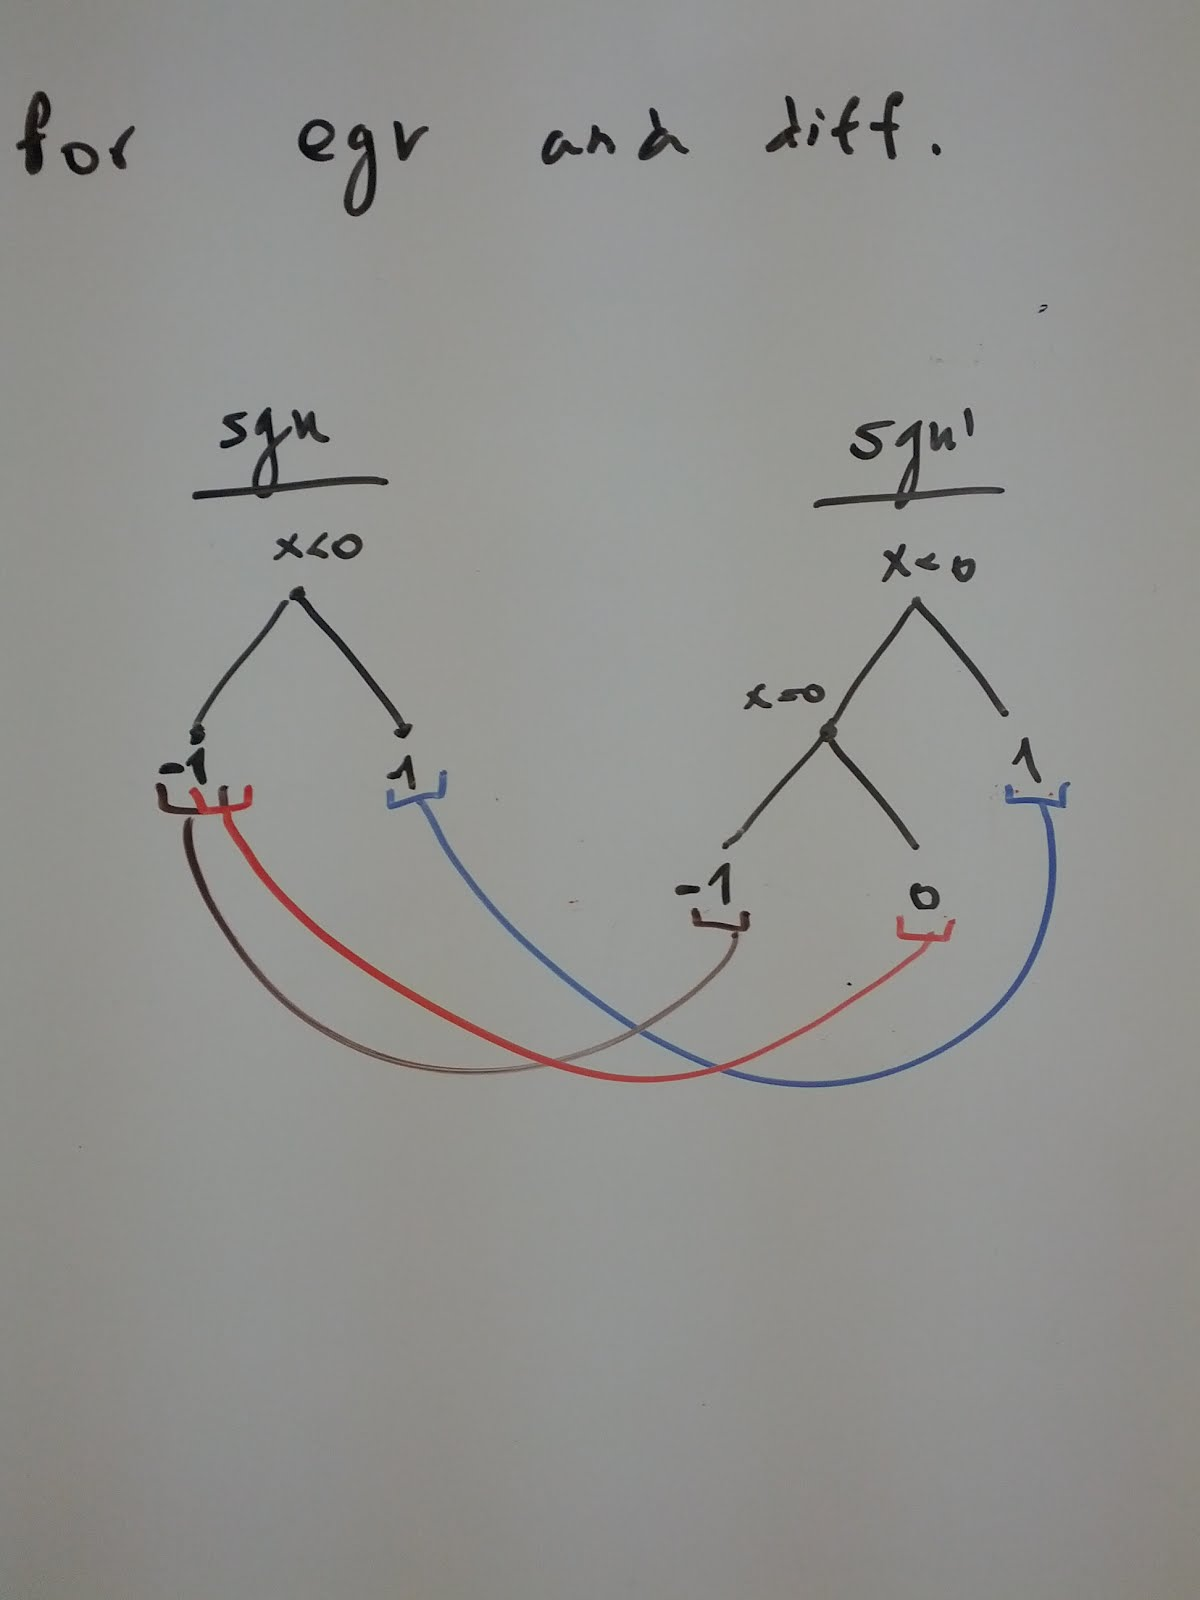
\includegraphics[scale=0.15,clip=true,trim = 125pt 450pt 100pt 350pt]{figures/sign-complete.jpg}
%}
%\caption{Complete disjunction analysis sound comparison for $sign$ and $sign'$}\figlabel{SignComplete}
%\end{wrapfigure}


Unfortunately, tracking correlations across such program would be hard, is it completely executes $P$ before reaching $P'$



Given two programs $P$ and $P'$, we can construct a ``union program'' by considering the sequential composition ($P;P'$) of $P$ and $P'$.

To establish equivalence, our abstraction would need to match corresponding paths in $P$ and $P'$. This requires an abstraction to maintain full path sensitivity across all of $P$ and then ...


%In some cases, it would have been sufficient to use alternative domains that are capable of representing richer information, such as interval polyhedra~\cite{CMWC:SAS09}, or other numerical domains that can represent non-convex information (e.g., \cite{TODO}). The recent donut domain~\cite{GIBMG:VMCAI12} may be of particular interest for this purpose. However, the general principle of having to preserve correlating information even when information about the values is abstracted away, holds in all of these cases.

%\begin{figure}
%\imagetop{
%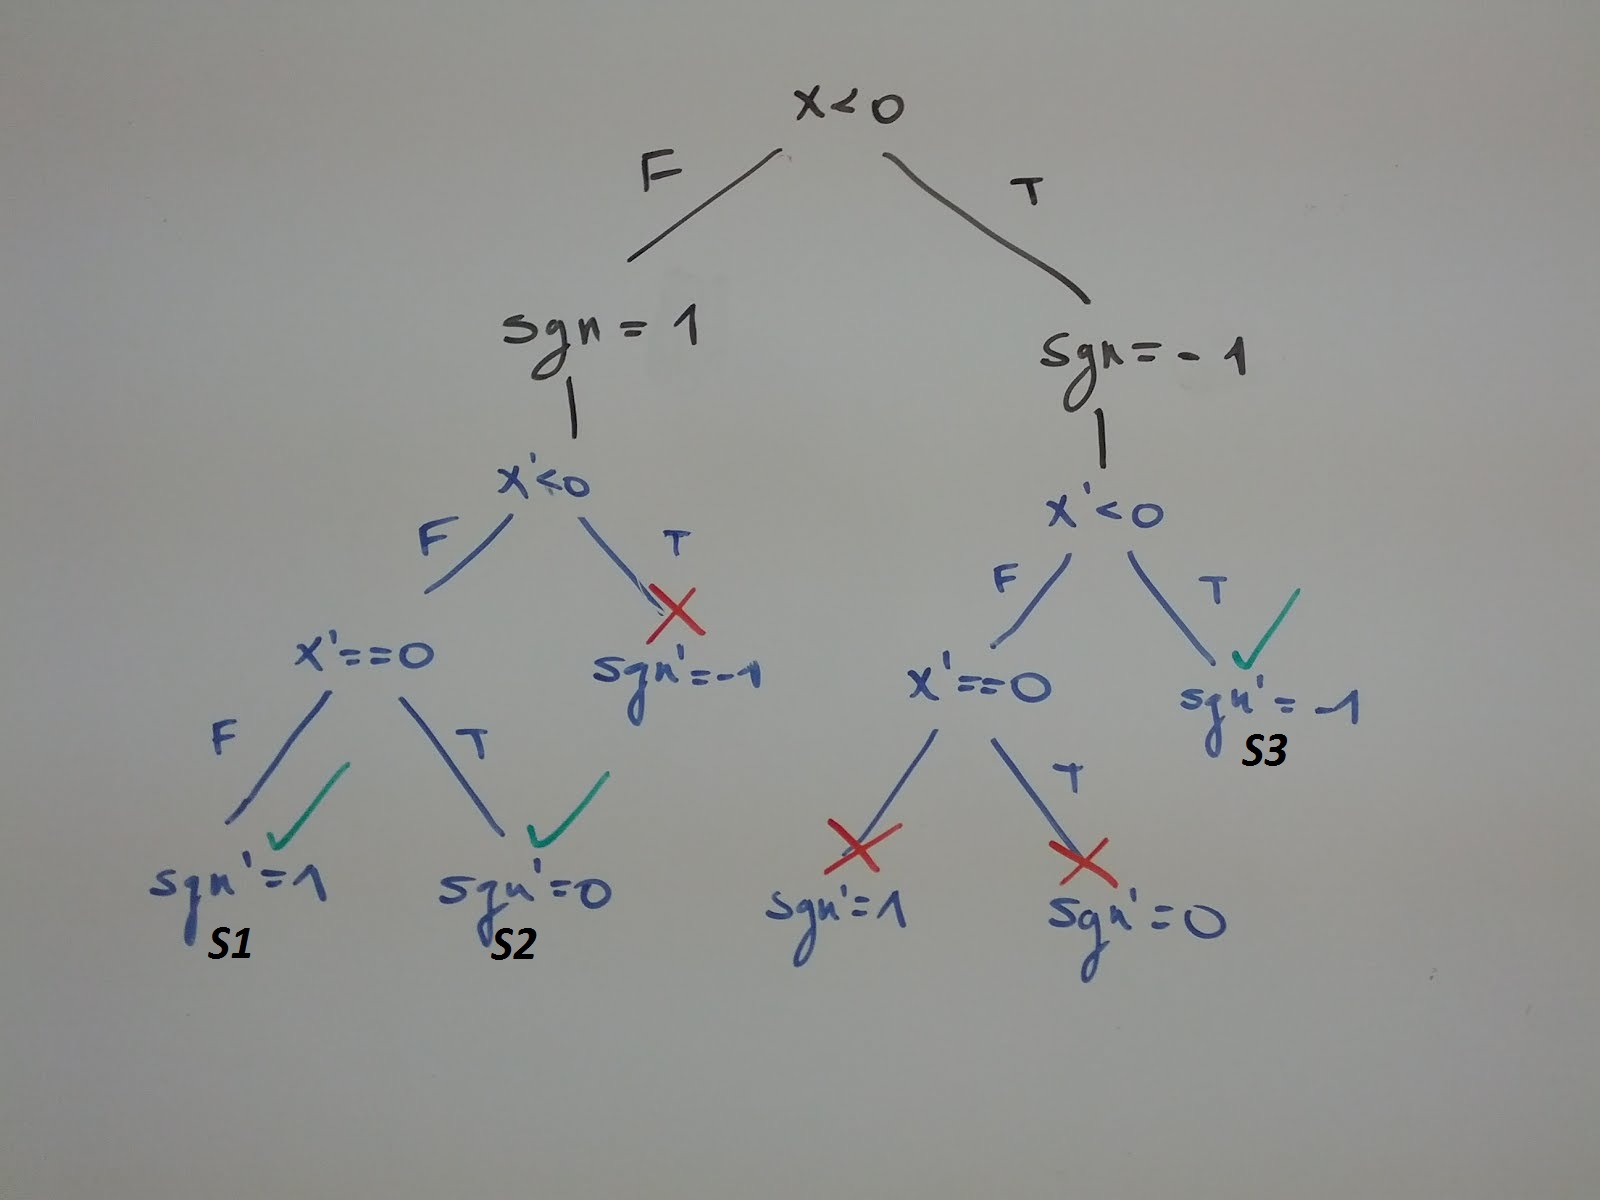
\includegraphics[scale=0.28,clip=true,trim = 50pt 100pt 100pt 0pt]{figures/sign-analysis1.jpg}
%}
%\caption{Joint $sign;sign'$ analysis}\figlabel{SignAnalysis1}
%\end{figure}

%However, analyzing over $P;P'$ means in the worst case remembering the states along each $P$-path and relating them to states in the corresponding $P'$-path. This approach is similar to the symbolic execution approach~\cite{} where all possible correlating paths are explored individually and output is examined to determine difference whilst attempting to reach full coverage. Much like this approach, this abstraction is unfeasible for most cases, especially for programs with an unbound number of paths e.g. \textbf{loops}. To avoid this we move to a partially disjunctive domain, partitioned by \emph{equivalence criteria}.
